%%%%%%%%%%%%%%%%%%%%%%%%%%%%%%%%%%%%%%%%%
% FRI Data Science_report LaTeX Template
% Version 1.0 (28/1/2020)
% 
% Jure Demšar (jure.demsar@fri.uni-lj.si)
%
% Based on MicromouseSymp article template by:
% Mathias Legrand (legrand.mathias@gmail.com) 
% With extensive modifications by:
% Antonio Valente (antonio.luis.valente@gmail.com)
%
% License:
% CC BY-NC-SA 3.0 (http://creativecommons.org/licenses/by-nc-sa/3.0/)
%
%%%%%%%%%%%%%%%%%%%%%%%%%%%%%%%%%%%%%%%%%


%----------------------------------------------------------------------------------------
%	PACKAGES AND OTHER DOCUMENT CONFIGURATIONS
%----------------------------------------------------------------------------------------
\documentclass[fleqn,moreauthors,10pt]{ds_report}
\usepackage[english]{babel}
\usepackage{xcolor}
\usepackage{tabularx}
\usepackage{listings}

\graphicspath{{fig/}}


\newcommand{\todo}[1]{\textcolor{red}{\textbf{#1}}}

%----------------------------------------------------------------------------------------
%	ARTICLE INFORMATION
%----------------------------------------------------------------------------------------

% Header
\JournalInfo{FRI Natural language processing course 2024}

% Interim or final report
\Archive{Project report} 
%\Archive{Final report} 

% Article title
\PaperTitle{Parameter-Efficient Fine-Tuning of Large Language Models} 

% Authors (student competitors) and their info
\Authors{Ondřej Komín, Andrej Sušnik, Eileen Vu}

% Advisors
\affiliation{\textit{Advisors: Slavko Žitnik}}

% Keywords
\Keywords{Keyword1, Keyword2, Keyword3 ...}
\newcommand{\keywordname}{Keywords}


%----------------------------------------------------------------------------------------
%	ABSTRACT
%----------------------------------------------------------------------------------------

\Abstract{This is the abstract}

%----------------------------------------------------------------------------------------

\begin{document}

% Makes all text pages the same height
\flushbottom 

% Print the title and abstract box
\maketitle 

% Removes page numbering from the first page
\thispagestyle{empty} 

%----------------------------------------------------------------------------------------
%	ARTICLE CONTENTS
%----------------------------------------------------------------------------------------
\section*{Introduction}
Since the introduction of attention \cite{vaswani2017attention}, using large language models (LLMs) such as Google's BERT \cite{devlin2019bert} and OpenAI's GPT \cite{radford2018gpt} has become inevitable to various applications across natural language processing (NLP) domains. These models have demonstrated remarkable capabilities in understanding and generating human-like text. However, to achieve optimal performance in specific tasks, fine-tuning these pre-trained models on task-specific data is often necessary.

This research paper focuses on presenting and comparing various parameter-efficient fine tuning (PEFT) methods in the context of optimizing natural language processing tasks. Through empirical experiments, we aim at exploring the effectiveness of different PEFT approaches in achieving desirable trade-offs between model complexity, computational efficiency, and task performance. Similarly to the work done in \cite{xu2023parameterefficient}, we begin our research by reviewing and categorizing popular PEFT methods. We continue by presenting and discussing the theoretical foundations of three specific methodologies and applying these to five different datasets that cover various natural language understanding skills. Lastly, the fine-tuned models will be evaluated based on appropriate performance metrics, computational resources required, and ease of adaptation to different tasks. Through this exploration, we aim at facilitating more resource-conscious approaches to model optimization, accelerating progress in the field of NLP and its applications.
%------------------------------------------------
\section*{Related Work}
Fine-tuning LLMs plays a crucial role in adapting these models to domain-specific tasks. As LLMs are pre-trained on vast amounts of text data, they capture linguistic patterns and semantic information. However, for tasks with specific requirements, such as sentiment analysis or named entity recognition, fine-tuning allows these models to tailor their representations to better suit the task at hand. 

Traditional methods of full fine-tuning involve updating all parameters of the pre-trained LLM. The popular GPT-4 model released in early 2024 contains 1.76 trillion weights \cite{openai2024gpt4}. Fine-tuning (and storing) this amount of parameters whenever one wants to apply the model to a specific use case however not only requires significant computational resources but also poses a risk of overfitting, especially in scenarios with limited task-specific data.

\noindent In order to avoid these problems, PEFT methods have emerged as a solution to the drawbacks of full fine-tuning. These methods aim to optimize neural networks with fewer parameters while maintaining comparable performance to traditional fine-tuning approaches. By reducing the number of parameters updated during fine-tuning, PEFT not only mitigates computational costs but also helps alleviate overfitting concerns. As described in \cite{xu2023parameterefficient}, PEFT techniques can be divided into five main categories: additive fine-tuning, partial fine-tuning, reparameterized fine-tuning, hybrid fine-tuning and lastly unified fine-tuning. While some of these methods aim at introducing new trainable parameters for use-case-specific fine-tuning, others reduce the number of trainable parameters by transforming the weights into lower dimensions.

In this paper, we focus on presenting and comparing three PEFT methods in the context of different NLP tasks. Specifically, we investigate the performance of the following methodologies: low rank adaptation (LoRA), soft prompt-based fine-tuning, and partial fine-tuning. \textbf{LoRA} \cite{hu2021lora} has become very popular in the last years due to its ability to reduce the number of parameters without introducing additional latency, unlike for example adapter methods. This lowers training computational requirements while improving performance for specific NLP tasks. \textbf{Soft-prompting} \cite{lester2021power} is a machine learning technique that offers subtle guidance to models during training, aiding in learning without the need for explicit labels. This approach is valuable as it allows for more flexible decision-making while still achieving desired outcomes, especially in scenarios where labeled data may be scarce or costly to obtain. Lastly, we will investigate the partial fine-tuning method \textbf{BitFit}\cite{zaken2022bitfit}. This method only fine-tunes the bias term of the layers while freezing the rest of the network. This technique, which trains less than 0.1\% of the total number of weights, was proven to achieve comparable performance than full fine-tuning.

\begin{table}[htbp]
  \centering
  \begin{tabularx}{\columnwidth}{lX}
    \toprule
    \textbf{Benchmark} & \textbf{NLP Task} \\
    \midrule
    CommonsenseQA \cite{talmor2019commonsenseqa} & Commonsense Reasoning \\
    CoNLL-2012 \cite{pradhan2012conll} & Coreference Resolution \\
    XSum \cite{narayan2018xsum} & Text Summarization \\
    SST5 \cite{maas2011sentiment} & Sentiment Analysis \\
    Slovene SuperGLUE \cite{robnik2022superglue} & Slovene BoolQ (Boolean Questions) \\
    \bottomrule
  \end{tabularx}
  \caption{Chosen benchmarks for performance evaluation}
  \label{tab:benchmarks}
\end{table}
We will provide an empirical comparison of these three methodologies based on five different NLP tasks. The benchmarks we have chosen for this each represent distinct natural language understanding skills allowing us to provide a comprehensive overview of the advantages and disadvantages of all techniques.
%------------------------------------------------
\section*{Methods}
% \todo{Eileen}
% \paragraph{BitFit} 
Bias-terms Fine-tuning (BitFit) \cite{zaken2022bitfit} is a parameter-efficient fine-tuning technique for pretrained language models that focuses on updating only the bias terms of the model's weights. This approach aims to reduce the computational and memory resources required for fine-tuning while maintaining performance on downstream tasks.

In BitFit, instead of updating all parameters $\mathbf{W}$ and $\mathbf{b}$, we update only the bias $\mathbf{b}$. The weights $\mathbf{W}$ remain fixed. During fine-tuning, the gradients are computed with respect to $\mathbf{b}$ only, and the updates are applied as follows:
\[
\mathbf{b} \leftarrow \mathbf{b} - \eta \frac{\partial \mathcal{L}}{\partial \mathbf{b}}
\]
where $\eta$ is the learning rate and $\mathcal{L}$ is the loss function.

BitFit has three key properties: it can match the results of a fully fine-tuned model, it enables tasks to arrive in a stream without requiring simultaneous access to all datasets, and it fine-tunes only a small portion of the model's parameters. Specifically, BitFit trains less than 0.1\% of the total number of parameters, yet it achieves transfer learning performance comparable to, and sometimes better than, fine-tuning the entire network.

\paragraph{Infused Adapter by Inhibiting and Amplifying Inner Activations (IA3)} The IA3 approach rescales inner activations with learned vectors. These learned vectors are injected in the attention and feedforward modules in a typical transformer-based architecture. These learned vectors are the only trainable parameters during fine-tuning, and thus the original weights remain frozen. Dealing with learned vectors (as opposed to learned low-rank updates to a weight matrix like LoRA) keeps the number of trainable parameters much smaller.

Similar to LoRA, IA3 offers several advantages: it efficiently reduces the number of trainable parameters, with IA3 models typically having only about 0.01\% trainable parameters for base models like T0, compared to over 0.1\% for LoRA. Additionally, IA3 maintains frozen pre-trained weights, allowing for the creation of multiple lightweight and portable models for various tasks. Despite its parameter efficiency, models fine-tuned using IA3 demonstrate performance comparable to fully fine-tuned models, without introducing any inference latency.

% \noindent\todo{Ondra} 
% \paragraph{LoRA}

LoRA \cite{hu2021lora} is a method designed for fine-tuning large models. It operates by fixing the weights of the original model and introducing a trainable low-rank decomposition matrix into the LLM architecture. This modified architecture involves fixing the original weights $W_0$ while introducing additional trainable weights $\Delta W$, which can be decomposed into matrices $BA$, where the rank of both $B$ and $A$ is much smaller than that of $W_0$. Consequently, the resulting weights are formulated as $W0 + BA$, significantly reducing the number of parameters that need to be trained. 

Empirical results indicate that LoRA performs comparably or even better than other methods, while requiring a comparable or lower number of trainable parameters. Notably, LoRA drastically reduces the number of trainable parameters, such as in the case of fine-tuning the GPT-3 model, where the parameter count was reduced by 10000 times, accompanied by a threefold reduction in GPU memory requirement. Additionally, LoRA exhibits several benefits, including the ability to train specialized models without introducing latency, as seen in adapter methods. 

Moreover, it enables the deployment of multiple specialized models simultaneously by reducing memory and computational footprint, achieved through maintaining fixed weights for the base model while having several trained decomposition matrices for each specialized task.

LoRa model is trained with configuration showed in Listing \ref{lst:lora_params}.

\begin{lstlisting}[language=Python, caption={LoRa parameters}, label={lst:lora_params}]
lora_config = LoraConfig(
        r=16,
        lora_alpha=32,
        lora_dropout=0.1,
        bias="lora_only",
        task_type="SEQ_CLS"
)
\end{lstlisting}

% \noindent\todo{Andrej} 
% \paragraph{Prompt Tuning}
% Prompt tuning\cite{lester2021power} is a process where users refine their input prompts to generate more accurate and relevant responses from AI models like GPT-3.5. It involves experimenting with different phrasings, keywords, and structures to guide the model towards desired outputs. By iteratively adjusting prompts, users can fine-tune the model's understanding and improve the quality of its responses for specific tasks or contexts. Prompt tuning is crucial for optimizing AI performance and tailoring its outputs to meet diverse needs effectively.
summarization of prompt tuning
%------------------------------------------------
% \section*{Model}
% Recommendation by Tutor: multilingual DeBERTA v3, sloBERTA, BERTIC (all Balkan languages), CROSLOBERTA
% Baseline: normal fine-tuning
% q Lora (half of the bits than LORA)

% other benchmarks: XGLUE (but our benchmarks should be fine)

% adapters
% - have one NN
% - have multiple adapters for each task
% - is implemented already

% next steps:
% - take slvoenian dataset
% - choose model
% - implement fine-tuning
% - use libraries if available

% until next time:
% - have three methods and finetuning impelemnted
% - for slovenian dataset
% %------------------------------------------------
\section*{Training Pipeline}
\begin{figure}[ht!]
    \centering
    {
\includegraphics[scale=0.5]{fig/training_pipieline.png}}
    \caption{Training Pipeline}
    \label{fig:pipeline}
\end{figure}

The training pipeline consists of five main steps, each applicable for the successful fine-tuning of the models for specific tasks. 

\paragraph{Step 1} Initially, we imports necessary libraries and set up the environment. Using custom dataset handlers, we load the datasets based on the specified task. 

\paragraph{Step 2} After loading the dataset, the we apply pre-processing functions tailored to the BERT tokenizer. This step involves tokenizing and encoding the text data, which is essential for input to the BERT model. The pre-processed data is split into train, validation, and test sets, and formatted as PyTorch tensors for compatibility with the BERT model.

\paragraph{Step 3} Next, we configure the training arguments, including parameters such as output directory, evaluation strategy, learning rate, batch size, and number of epochs. It also initializes the BERT model for the task and defines the trainers for the different methods. Each trainer is associated with its specific model path and training configurations.
\begin{lstlisting}[language=Python, caption={Training Arguments}, label={lst:training_arguments}]
args = TrainingArguments(
    output_dir=model_path,
    evaluation_strategy="epoch",
    learning_rate=2e-5,
    per_device_train_batch_size=64,
    per_device_eval_batch_size=64,
    auto_find_batch_size=True,
    num_train_epochs=20,
    weight_decay=0.01,
)
\end{lstlisting}



\paragraph{Step 4} With the trainers defined, we execute the training process for all PEFT methods. This step involves fine-tuning the BERT model on the data using the specified training arguments and data. 

\paragraph{Step 5} Finally, we evaluate the trained models using the evaluation datasets. Performance metrics such as accuracy, precision, F1-score, and recall are computed for the different methods. The results are compared to assess the effectiveness of each fine-tuning approach on specific tast.

%------------------------------------------------
\section*{Environment and reproducibility}
We ran the experiments on the Arnes cluster, the compute node that we used included AMD EPYC™ 9124 CPU, 256GB of RAM and NVIDIA H100 GPU. The cluster uses SLURM middleware for it's job managment and we used sbatch command to run our jobs. To have reproducible environment we used containerization with Apptainer. Apptainer is a containerization solution mainly used in high performance computing. We used Python version 3.12 and we have gathered all the requirements into requirements.txt file and specified the versions of the packages. The source code is available in the repository\footnote{\url{https://github.com/UL-FRI-NLP-2023-2024/ul-fri-nlp-course-project-naturallylazypeople}}. Results can be reproduced by logging into the supercomputer cluster of your choice, cloning the repository and executing following commands.

\begin{lstlisting}[language=bash,caption={Commands for running the training and evaluation}]
cd src
sbatch run.sh
\end{lstlisting}

Sbatch command will put job in the SLURM queue. After the job is accepted Apptainer container with the environment will be built. When the environment is built, the main script will be executed inside the containerized environment, firstly all the models will be trained and the evaluated.
% \subsection{Hardware Configuration}
% \begin{itemize}
%     \item \textbf{Central Processing Unit (CPU):} AMD EPYC™ 9124
%     \item \textbf{Random Access Memory (RAM):} 256GB
%     \item \textbf{Graphics Processing Unit (GPU):} Nvidia H100
% \end{itemize}

% \subsection{Software Configuration}
% \begin{itemize}
%     \item \textbf{Job Scheduling and Resource Management:} SLURM (Simple Linux Utility for Resource Management)
%     \item \textbf{Containerization Platform:} Apptainer
%     \item \textbf{Programming Language:} Python (version not specified)
%     \item \textbf{Python Dependencies:} Listed in \texttt{requirements.txt}
% \end{itemize}

% \subsection{Description}
% The computational environment comprises robust hardware components, including the AMD EPYC™ 9124 CPU, providing high-performance computing capabilities, supported by ample memory resources with 256GB of RAM, and enhanced computational capabilities with the inclusion of the Nvidia H100 GPU.

% To manage computational tasks efficiently, SLURM (Simple Linux Utility for Resource Management) is employed for job scheduling and resource allocation across the cluster infrastructure. Additionally, the Apptainer containerization platform is utilized to encapsulate applications and their dependencies, ensuring reproducibility and portability of computational workflows.

% Python serves as the primary programming language within this environment, facilitating a wide range of scientific and computational tasks. To maintain reproducibility, the specific dependencies and versions of Python packages are documented in the \texttt{requirements.txt} file, ensuring consistency and replicability of computational experiments and analyses.

%------------------------------------------------
\section*{Results}
\paragraph{CommonsenseQA} The CommonsenseQA dataset is a benchmark designed to evaluate AI systems on commonsense reasoning. It consists of multiple-choice questions, each with five answer options and one correct answer. The questions cover various aspects of commonsense knowledge, such as physical properties, social behaviors, causal relationships, and temporal and spatial reasoning.

The CommonsenseQA dataset consists of multiple-choice questions, each with five answer options (labeled A to E), one of which is correct. The correct answer is annotated for each question. The dataset is designed to challenge AI models to develop a deeper understanding of the world, similar to human commonsense reasoning. It is used to evaluate natural language understanding models, develop and benchmark new AI algorithms, and study AI's limitations and capabilities in understanding everyday scenarios. The CommonsenseQA dataset presents challenges such as handling ambiguity, context-dependence, and requiring complex reasoning.

We finetuned the mdeberta-small model. We can see that when using LoRa PEFT method we can achieve almost the same performance than with full finetuning while requiring much less training time. The BitFit method does not give a good result for this dataset.

\begin{table}[htbp]
  \centering
  \begin{tabularx}{\columnwidth}{@{} l *{3}{X} @{}}
    \toprule
    \textbf{Metric} & \textbf{FFT} & \textbf{LoRA} & \textbf{BitFit} \\
    \midrule
    Batch Size & 64 & 128 & 128 \\
    Training Time [sec] & 5798 & 4523 & 4539 \\
    RAM Usage [MB] & 1998 & 2002 & 2005 \\
    \# Parameters [$\times 10^6$] & 14 & 0.03 & 0.033 \\
    Accuracy & 0.66 & 0.65 & 0.42 \\
    Precision & 0.66 & 0.65 & 0.42 \\
    F1-Score & 0.66 & 0.65 & 0.42 \\
    Recall & 0.66 & 0.65 & 0.43 \\
    \bottomrule
  \end{tabularx}
  \caption{Performance of Full Finetuning vs PEFT methods on CommonsenseQA}
  \label{tab:comparison}
\end{table}

\paragraph{CoNLL-2012} We will continue our analysis with the task of coreference resolution. Coreference resolution is the task of identifying when different expressions in a text refer to the same entity. The CoNLL-2012 shared task \footnote{\url{https://huggingface.co/datasets/conll2012_ontonotesv5}} is a benchmark dataset and competition for coreference resolution  which provides annotated data where entities are linked across sentences, helping models learn to recognize these relationships. We will fine-tune an mDeBERTa model of type DebertaForTokenClassification, i.e. a model with a token classification head suitable for coreference resolution tasks.

Pre-processing for coreference resolution is quite different from pre-processing in the context of text classification. While text classification assigns a single label to an entire text (e.g. A or B), coreference resolution assigns labels to individual tokens to indicate their membership in coreference chains, which group tokens referring to the same entity. During tokenization, it is crucial to align these labels with the tokenized output. Furthermore, padding ensures consistent length for all token sequences. Tokens without corresponding coreference labels are padded with a special token to maintain alignment and indicate they do not belong to any coreference chain. This method accurately prepares the dataset for training a model to resolve coreferences in text.
\begin{table}[htbp]
    \centering
    \resizebox{\columnwidth}{!}{%
    \begin{tabular}{@{}llllll@{}}
    \toprule
    \textbf{Metric} & \textbf{FFT} & \textbf{LoRA} & \textbf{Soft Prompts} & \textbf{IA3} & \textbf{BitFit} \\ \midrule
    Batch Size & 64 & 128 & 128 & 128 & 128 \\
    Training Time [sec] & 2129 & 1803 & 1881 & 1799 & 1788 \\
    RAM Usage [MB] & 2291 & 2302 & 2341 & 2341 & 2342 \\
    \# Parameters [$\times 10^6$] & 183.86 & 0.64 & 0.05 & 0.06 & 0.10 \\
    Accuracy & 0.76 & 0.78 & 0.79 & 0.78 & 0.77 \\
    Precision & 0.64 & 0.61 & 0.63 & 0.61 & 0.61 \\
    F1-Score & 0.69 & 0.68 & 0.70 & 0.68 & 0.68 \\
    Recall & 0.76 & 0.78 & 0.79 & 0.78 & 0.77 \\
    \bottomrule
    \end{tabular}}
    \caption{Performance of Full Finetuning vs PEFT methods on CoNLL-2012 for mDeBERTa-base}
\end{table} Compared to Full Fine-Tuning, the PEFT methods dramatically reduce training time and memory usage. Despite their efficiency, PEFT methods achieve comparable, and in some cases superior results. Among the PEFT methods evaluated, Soft Prompts performed the best overall. It achieved the highest accuracy and recall, indicating it can identify correct answers more effectively and consistently. It even outperforms full-fine-tuning. Additionally, Soft Prompts had the second lowest RAM usage and a minimal number of trainable parameters, underscoring its efficiency. 

If we compare the above results for mDeBERTa-base with the below results for mDeBERTa-small, we notice that the training time and RAM usage are significantly smaller for the mDeBERTa-small model. However, despite the smaller model size and reduced resource requirements, the performance in terms of accuracy, precision, recall, and F1-score remains similar between the two models. This suggests that the mDeBERTa-small model offers a more resource-efficient alternative without compromising on performance compared to the larger mDeBERTa-base model.

\begin{table}[htbp]
    \centering
    \resizebox{\columnwidth}{!}{%
    \begin{tabular}{@{}llllll@{}}
    \toprule
    \textbf{Metric} & \textbf{FFT} & \textbf{LoRA} & \textbf{Soft Prompts} & \textbf{IA3} & \textbf{BitFit} \\ \midrule
    Batch Size & 64 & 128 & 128 & 128 & 128 \\
    Training Time [sec] & 1114 & 971 & 1060 & 951 & 958 \\
    RAM Usage [MB] & 1926 & 1928 & 2024 & 2100 & 2094 \\
    \# Parameters [$\times 10^6$] & 141.34 & 0.34 & 0.05 & 0.05 & 0.05 \\
    Accuracy & 0.77 & 0.77 & 0.78 & 0.77 & 0.63 \\
    Precision & 0.63 & 0.61 & 0.62 & 0.61 & 0.40 \\
    F1-Score & 0.69 & 0.68 & 0.69 & 0.68 & 0.49 \\
    Recall & 0.77 & 0.77 & 0.78 & 0.77 & 0.63 \\
    \bottomrule
    \end{tabular}}
    \caption{Performance of Full Finetuning vs PEFT methods on CoNLL-2012 for mDeBERTa-small}
    \label{tab:comparison}
\end{table}

\paragraph{Slovene SuperGLUE} While most of the research in the field of NLP has been conducted for the English language, we also aim at applying the PEFT methods to multilingual text reasoning. The benchmark used is the Slovene SuperGLUE \cite{robnik2022superglue}, which is the Slovene version of the English SuperGLUE. The benchmark consists of eight tasks encompassing general NLP tasks. Let us begin with the task BoolQ: a dataset with questions and binary answers \footnote{\url{https://huggingface.co/datasets/google/boolq}}. Each instance consists of three components: a question, a passage, and an answer, with the possibility of including the page title as supplementary context. This configuration mirrors the structure of typical natural language inference tasks focused on text pairs.

We employed an mDeBERTa model, see Table \ref{tab:superglue-mdeberta}, as well as a BERTić \cite{ljubesic2021bertic} model, see Table \ref{tab:superglue-bertic}, for fine-tuning, which is a transformer language model specifically designed for Bosnian, Croatian, Montenegrin, and Serbian. Note that for BERTić, we had resources on the shared cluster for training only LoRA and FFT.

\begin{table}[htbp]
  \centering
  \label{tab:comparison}
  \resizebox{\columnwidth}{!}{%
    \begin{tabular}{@{}lllll@{}}
    \toprule
    \textbf{Metric} & \textbf{FFT} & \textbf{LoRA} & \textbf{Soft Prompts} & \textbf{BitFit} \\ \midrule
    Batch Size & 64 & 128 & 128 & 128 \\
    Training Time [sec] & 5282 & 4478 & 4567 & 4456 \\
    RAM Usage [MB] & 2337 & 2338 & 2338 & 2337 \\
    \# Parameters [$\times 10^6$] & 278.6 & 0.62 & 0.16 & 0.1 \\
    Accuracy & 0.7 & 0.63 & 0.62 & 0.65 \\
    Precision & 0.74 & 0.78 & 0.62 & 0.62 \\
    F1-Score & 0.77 & 0.72 & 0.76 & 0.76 \\
    Recall & 0.81 & 0.77 & 1.0 & 1.0 \\
    \bottomrule
    \end{tabular}}
    \caption{Performance of Full Finetuning vs PEFT methods on Slovene SuperGLUE for mDeBERTa-base}
    \label{tab:superglue-mdeberta}
\end{table}

\begin{table}[htbp]
  \centering
  \begin{tabularx}{\columnwidth}{@{} l *{3}{X} @{}}
    \toprule
    \textbf{Metric} & \textbf{FFT} & \textbf{LoRA} \\ \midrule
    Batch Size & 64 & 128\\
    Training Time [sec] & 3967 & 3277\\
    RAM Usage [MB] & 761 & 458\\
    \# Parameters [$\times 10^6$] & 110.6 & 1.2\\
    Accuracy & 0.74 & 0.65\\
    Precision & 0.78 & 0.71\\
    F1-Score & 0.79 & 0.73\\
    Recall & 0.81 & 0.75\\
    \bottomrule
  \end{tabularx}
  \caption{Performance of Full Finetuning vs LoRA on Slovene SuperGLUE for BERTić}
  \label{tab:superglue-bertic}
\end{table}

For mDeBERTa, the LoRA technique stands out with significantly lower RAM usage and a remarkable reduction in the number of parameters compared to full fine-tuning, while maintaining competitive performance. On the other hand, Soft Prompts and BitFit show promising results in terms of accuracy and precision, although they require slightly more training time and memory resources. For BERTić, the LoRA method also demonstrates a substantial reduction in RAM usage and parameter count, with a notable improvement in precision compared to full fine-tuning. These findings suggest that LoRA could be a viable option for enhancing model efficiency without compromising task performance across different languages and models.

\paragraph{SST-5} dataset (also known as Stanford Sentiment Treebank with 5 labels) was created to test model's capacity for sentiment classification. It contains 11855 sentences from movie reviews labeled by human judges. Label of the review can be one of the five classes - negative, somewhat negative, neutral, somewhat positive and positive. Therefore the dataset is sometimes also referred as SST fine-graned. 

Before tokenizing sentences for the model we do basic preprocessing which involves removal of special characters, conversion to lower case and removal of stopwords.

For this dataset we employed Deberta model for classification. Results of the finetuning can be seen in Table \ref{tab:sst5_deberta_base}. Lora seems to be performing the best out of all peft methods, regarding accuracy and recall. Other metrics are slightly better or comparable with the other peft methods.

\begin{table}[htbp]
  \centering
  \resizebox{\columnwidth}{!}{%
    \begin{tabular}{@{}llllll@{}}
    \toprule
    \textbf{Metric} & \textbf{FFT} & \textbf{LoRA} & \textbf{IA3} & \textbf{BitFit} \\ \midrule
    Batch Size & 64 & 128 & 128 & 128 \\
    Training Time [sec] & 663 & 542 & 548 & 531 \\
    RAM Usage [MB] & 1979 & 2105 & 2105 & 2105 \\
    \# Parameters [$\times 10^6$] & 184.43 & 0.61 & 0.07 & 0.10 \\
    Accuracy & 0.52 & 0.42 & 0.25 & 0.25 \\
    Precision & 0.52 & 0.22 & 0.2 & 0.06 \\
    F1-Score & 0.51 & 0.29 & 0.2 & 0.06 \\
    Recall & 0.52 & 0.42 & 0.25 & 0.25 \\
    \bottomrule
    \end{tabular}}
    \caption{Performance of Full Finetuning vs PEFT methods on SST5 for mDEBERTA-base}
    \label{tab:sst5_deberta_base}
\end{table}
%------------------------------------------------
\section*{Future directions, ideas}
In the future we want to focus on other PEFT method, \textit{BitFit} and \textit{Prompt Tuning}. 

Other direction of our work will be to broaden selection of benchmarks on which we test the methods.

Lastly, we may do more in depth hyperparameter tuning regarding each model, e.g. with LoRa try different matrix ranks, etc.
%------------------------------------------------
\section*{Discussion}
% Use the Discussion section to objectively evaluate your work, do not just put praise on everything you did, be critical and exposes flaws and weaknesses of your solution. You can also explain what you would do differently if you would be able to start again and what upgrades could be done on the project in the future.
%------------------------------------------------
% \section*{Backup}
% In general, PEFT methods can be divided into five main categories \cite{xu2023parameterefficient}:
\begin{enumerate}
    \item \textbf{additive fine-tuning}: these methods introduce new extra trainable parameters for task-specific fine-tuning. One can further divide into the following subcategories:
    \begin{enumerate}
        \item \textbf{Adapter-based Fine-tuning}: an adapter module is incorporated into the transformer, allowing for fine-tuning without modifying the pretrained parameters 
        \item \textbf{Soft Prompt-based Fine-tuning}: trainable continuous vectors, known as soft prompts, are inserted into the input or hidden state of the model. Unlike manually designed hard prompts, soft prompts are generated by searching for prompts in a discrete token space based on task-specific training data 
        \item \textbf{Others} 
    \end{enumerate}
    \item \textbf{Partial Fine-tuning}: aims at reducing the number of fine-tuned parameters by selecting a subset of pre-trained parameters that are critical to downstream tasks while discarding unimportant ones. We further differentiate between: 
    \begin{enumerate}
        \item \textbf{Bias Update}: only the bias term in the attention layer, feed-forward layer and layer normalization of the transformer is updated
        \item \textbf{Pretrained Weight Masking}: where the pretrained weights are masked using various pruning criterion
        \item \textbf{Delta Weight Masking}: delta weights are masked via pruning techniques and optimization approximation
    \end{enumerate}
    \item \textbf{Reparameterized Fine-tuning}: these methods utilize low-rank transformation to reduce the number of trainable parameters while allowing operating with high-dimensional matrices (e.g., pretrained weights)
    \begin{enumerate}
        \item \textbf{Low-rank Decomposition}: finds a lower rank matrix that captures the essential information of the original matrix while reducing computational complexity and memory usage by re-parameterizing the updated delta weight
        \item \textbf{LoRA Derivatives}: series of PEFT methods that are improved based on LoRA
    \end{enumerate}
    \item \textbf{Hybrid Fine-Tuning}: methods that aim to combine various PEFT approaches, such as adapter, prefix-tuning, and LoRA, to leverage the strengths of each method and mitigate their weaknesses
    \begin{enumerate}
        \item \textbf{Manual Combination}: mainly involves integrating the structure or features of one PEFT method into another PEFT method to enhance performance while achieving parameter efficiency
        \item \textbf{Automatic Combination}: explores how to configure PEFT methods like adapters, prefix-tuning, BitFit, and LoRA to different layers of the transformers automatically using various structure search and optimization approaches
    \end{enumerate}
    \item \textbf{Unified Fine-tuning}: lastly there are unified frameworks for fine-tuning, which streamlines the incorporation of diverse fine-tuning methods into a cohesive architecture, ensuring consistency and efficiency across the adaptation and optimization of models. Unlike hybrid fine-tuning methods, unified fine-tuning methods typically utilize a single PEFT method rather than a combination of various PEFT methods.
\end{enumerate}

% --------------BITFIT--------------

\noindent\todo{Eileen} \cite{zaken2022bitfit} BitFit Overview:
\begin{itemize}
    \item only the bias-terms of the model (or a subset of them) are being modified
    \item  freezing most of the network and fine-tuning only the bias-terms is surprisingly effective
    \item Three key properties
    \begin{enumerate}
        \item match the results of fully fine-tuned model
        \item enable tasks to arrive in a stream, this way it does not require simultaneous access to all datasets
        \item  fine-tune only a small portion of the model’s parameters
    \end{enumerate}
    \item trains less than 0.1\% of the total number of parameters
    \item Bitfit achieves transfer learning performance which is comparable (and sometimes better!) than fine-tuning of the entire network
\end{itemize}


% --------------LORA--------------

\textbf{Low Rank Adaptation (LoRA)} \cite{hu2021lora} is another PEFT method for fine tuning LLMs. Main principle behind LoRA is fixing the weights of the original model and then injecting trainable low rank decomposition matrix into the current LLM architecture. 

\begin{enumerate}
    \item \textbf{Architecture of the LoRA}

    Architecture of model is modified in following way. The original weights $W_{0}$ are fixed and additional trainable weights $\Delta W$ are introduced. $\Delta W$ can be decomposed to $BA$, where rank of both matrices $B$ and $A$ is much smaller than rank of the original $W_{0}$. Resulting weights are constructed as composition $W_{0} + \Delta W = W_{0} + BA$. This way much lower number of parameters is needed to be trained. Graphical depiction can be seen in Figure ~\ref{fig:LoRA}.

    \begin{figure}[h!]
        \centering
        {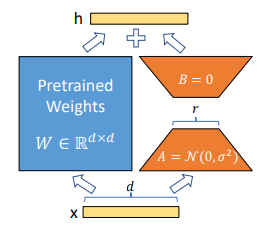
\includegraphics[scale=0.9]{imgs/LoRA.png}}
        \caption{schematic architecture of LoRa \cite{hu2021lora}}
        \label{fig:LoRA}
    \end{figure}
    
    \item \textbf{Empirical results}
    
    It turns out that LoRA performs similarly or even outperforms other methods compared in the paper, while having comparable or lower number of trainable parameters.
    For example comparing full finetuning of GPT-3 model with LoRA finetuning of the same model, the number of trainable parameters was reduced 10000 times and GPU memory requirement was reduced 3 times.
    
    Authors of the paper also noted that surprisingly low rank (as low as 1) is already yielding good results.
    
    \item \textbf{LoRA benefits}
    
    \begin{itemize}
        \item having relatively small amount of parameters to train
        \item not introducing additional latency, unlike e.g. adapter methods
        \item being able to deploy several specialized models at once, as LoRA reduces memory and computational footprint. LoRA does this by having several trained decomposition matrices for each specialized task while keeping the weights for the base model fixed.
    \end{itemize}
\end{enumerate}


% --------------PROMPT TUNING--------------

\textbf{The power of Scale for Parameter-Efficient Prompt Tunning}\cite{lester2021power} presents prompt tuning as an effective mechanism for conditioning frozen language models to perform specific tasks. The paper shows that prompt tuned T5-XXL model outperforms GPT-3 175B in SuperGLUE benchmark, despite having 16 times less parameters.


General overview:

\begin{itemize}
    \item definition of prompt tuning in the context of T5 fine tuning
    \item propose three options for initialization of prompt initialization and try different prompt lengths
    \item propose three methods for unlearning span corruption
    \item describe the results for different parameters
\end{itemize}

\begin{enumerate}
    \item \textbf{Prompt Tuning}
    
    Instead of modeling classification as the probability $Pr(y|X)$, it is modeled as $Pr(Y|X)$, where y is a single class label, Y is a sequence of tokens that represent a class label and X is a series of tokens. In T5 models in particular it is modeled as $Pr_\theta(Y|X)$
    When using prompt tuning the we use a $Pr_{\theta;\theta_p}(Y|[P;X])$ where P are prompt tokens. Models are trained to maximize the probability of Y, but only prompt parameters are updated.
    \begin{enumerate}
        \item \textbf{Design Decisions:} there are many ways of initializing the prompt representations. One possibility is training from scratch using random initialization. Better option is to initialize each prompt token to an embedding from models vocabulary. For classification tasks prompts could be initialized as embeddings that enumerate the output classes.
        \item \textbf{Unlearning Span Corruption:} span corruption could be a major problem of T5 model, so the paper describes experiments with three settings. "Span Corruption" uses pre-trained T5 as a frozen model. "Span Corruption + Sentinel" uses the same model but preappends setinels to all downstream targets. "LM Adaptation" continues with T5 self-supervised training for small number of additional steps, given a natural text prefix as input. LM adaptation transforms T5 into model more like GPT-3.
    \end{enumerate}
    \item  \textbf{Results}
    
    Frozen models ar built on top of pre-trained T5 checkpoints. The preformance is measured no SuperGLUE benchmark, each of the prompts is trained on a single SuperGLUE task. Prompts are tranied for 30000 steps using cross-entropy loss with a constant learning rate  of 0.3 and batch size of 32.
    \begin{enumerate}
        \item \textbf{Closing th Gap:} Prompt tuning becomes more competitive with model tuning as scale increases. When comparing with GPT-3 few shot preformance on SuperGLUE it is shown that T5-Small outperforms GPT-3 XL that is over 16 times larger.
        \item \textbf{Abation Study:}
        \begin{enumerate}
            \item Prompt lengths of sizes \{1, 5, 20, 100, 150\} were used, values above 20 produced only marginal increases
            \item Prompt initialization: for random initialization they sample uniformly from range [-0.5, 0.5]. For initialization from sampled vocabulary they restrict to 5000 most common tokens in T5's vocabulary. For "class label" initialization they take embeddings for the string representations of each class in downstream task. 
            \item Pre-training objective. The "span corruption" objective is not well suited for training frozen models and adding sentinels has little benefit. LM adaptation adds value across all model sizes.
        \end{enumerate}
    \end{enumerate}
\end{enumerate}
%----------------------------------------------------------------------------------------
%	REFERENCE LIST
%----------------------------------------------------------------------------------------
\bibliographystyle{unsrt}
\bibliography{report}

\end{document}